% chktex-file 24

\chapter{Theoretische Grundlagen}

\section{Business Process Model and Notation 2.0}

Business Process Model and Notation (BPMN 2.0)\cite{omg2014bpmn2} ist eine standardisierte grafische Sprache, 
die verwendet wird, um Geschäftsprozesse so zu dokumentieren, dass sie sowohl für Fachanwender 
als auch für technische Entwickler leicht verständlich sind. 
Ähnlich wie ein Architekt Baupläne nutzt, um Gebäude darzustellen, verwenden Business-Analysten 
BPMN 2.0, um visuelle Darstellungen organisatorischer Arbeitsabläufe und Abläufe zu erstellen.

BPMN-2.0-Diagramme\cite{omg2014bpmn2} zeigen die Abfolge von Geschäftstätigkeiten von Anfang bis Ende, 
einschließlich was passiert, wann es passiert und wer jede Aufgabe ausführt. Ein Beispiel: 
Ein Kundenbestellprozess könnte mit dem Eingang einer Bestellung beginnen, eine 
Lagerbestandsprüfung und Zahlungsabwicklung durchlaufen und mit dem Versand des Produkts enden.

\begin{enumerate}
    \item \textbf{Pools and Lanes:}
    \begin{itemize}
        \item \textbf{Pools} repräsentieren Teilnehmer eines Geschäftsprozesses, z. B. eine gesamte Organisation, eine Abteilung oder eine Rolle.
        \item \textbf{Lanes} sind Unterteilungen innerhalb von Pools, die spezifische Rollen oder Abteilungen darstellen. Sie helfen, Verantwortlichkeiten zu klären und den Prozess übersichtlich zu strukturieren.
    \end{itemize}

    \item \textbf{Activities:}
    \begin{itemize}
        \item \textbf{Tasks}: Abgrenzbare Arbeitsschritte, die nicht weiter unterteilt werden können.
        \item \textbf{Sub-Processes}: Komplexe Aktivitäten, die in mehrere Tasks unterteilt werden können und eigene detaillierte Abläufe enthalten.
        \item \textbf{Call Activities}: Verweise auf wiederverwendbare Prozesse oder Sub-Prozesse, die an anderer Stelle definiert sind.
    \end{itemize}

    \item \textbf{Events:}
    \begin{itemize}
        \item \textbf{Start Events}: Beginn eines Prozesses.
        \item \textbf{Intermediate Events}: Auftretende Ereignisse während des Prozesses, die den Ablauf beeinflussen können.
        \item \textbf{End Events}: Beenden eines Prozesses.
        \item \textbf{Message Events, Timer Events, Error Events, Conditional Events}: Spezialisierte Ereignisse, die Nachrichten, Zeitpläne, Fehler oder Bedingungen repräsentieren.
    \end{itemize}

    \item \textbf{Gateways:}
    \begin{itemize}
        \item \textbf{Exclusive Gateway (XOR)}: Nur ein Pfad wird gewählt.
        \item \textbf{Parallel Gateway (AND)}: Alle Pfade werden gleichzeitig durchlaufen.
        \item \textbf{Inclusive Gateway (OR)}: Einer oder mehrere Pfade werden durchlaufen.
        \item \textbf{Event-based Gateway}: Entscheidung basierend auf einem Ereignis.
    \end{itemize}

    \item \textbf{Flows:}
    \begin{itemize}
        \item \textbf{Sequence Flows}: Abfolge von Aktivitäten innerhalb eines Pools.
        \item \textbf{Message Flows}: Kommunikation zwischen Pools oder Prozessbeteiligten.
        \item \textbf{Association Flows}: Verknüpfung von Artefakten oder Datenobjekten mit Aktivitäten.
    \end{itemize}

    \item \textbf{Data Objects:}  
    Repräsentieren Informationen, die in einem Prozess verwendet oder erzeugt werden, z. B. Dokumente, Datenbanken oder Formulare.

    \item \textbf{Artifacts:}  
    Zusätzliche Elemente zur Prozessdokumentation, wie \textit{Groups} (zur visuellen Gruppierung) oder \textit{Text Annotations} (Kommentare oder Beschreibungen).

\end{enumerate}

\begin{figure}[ht]
    \centering
    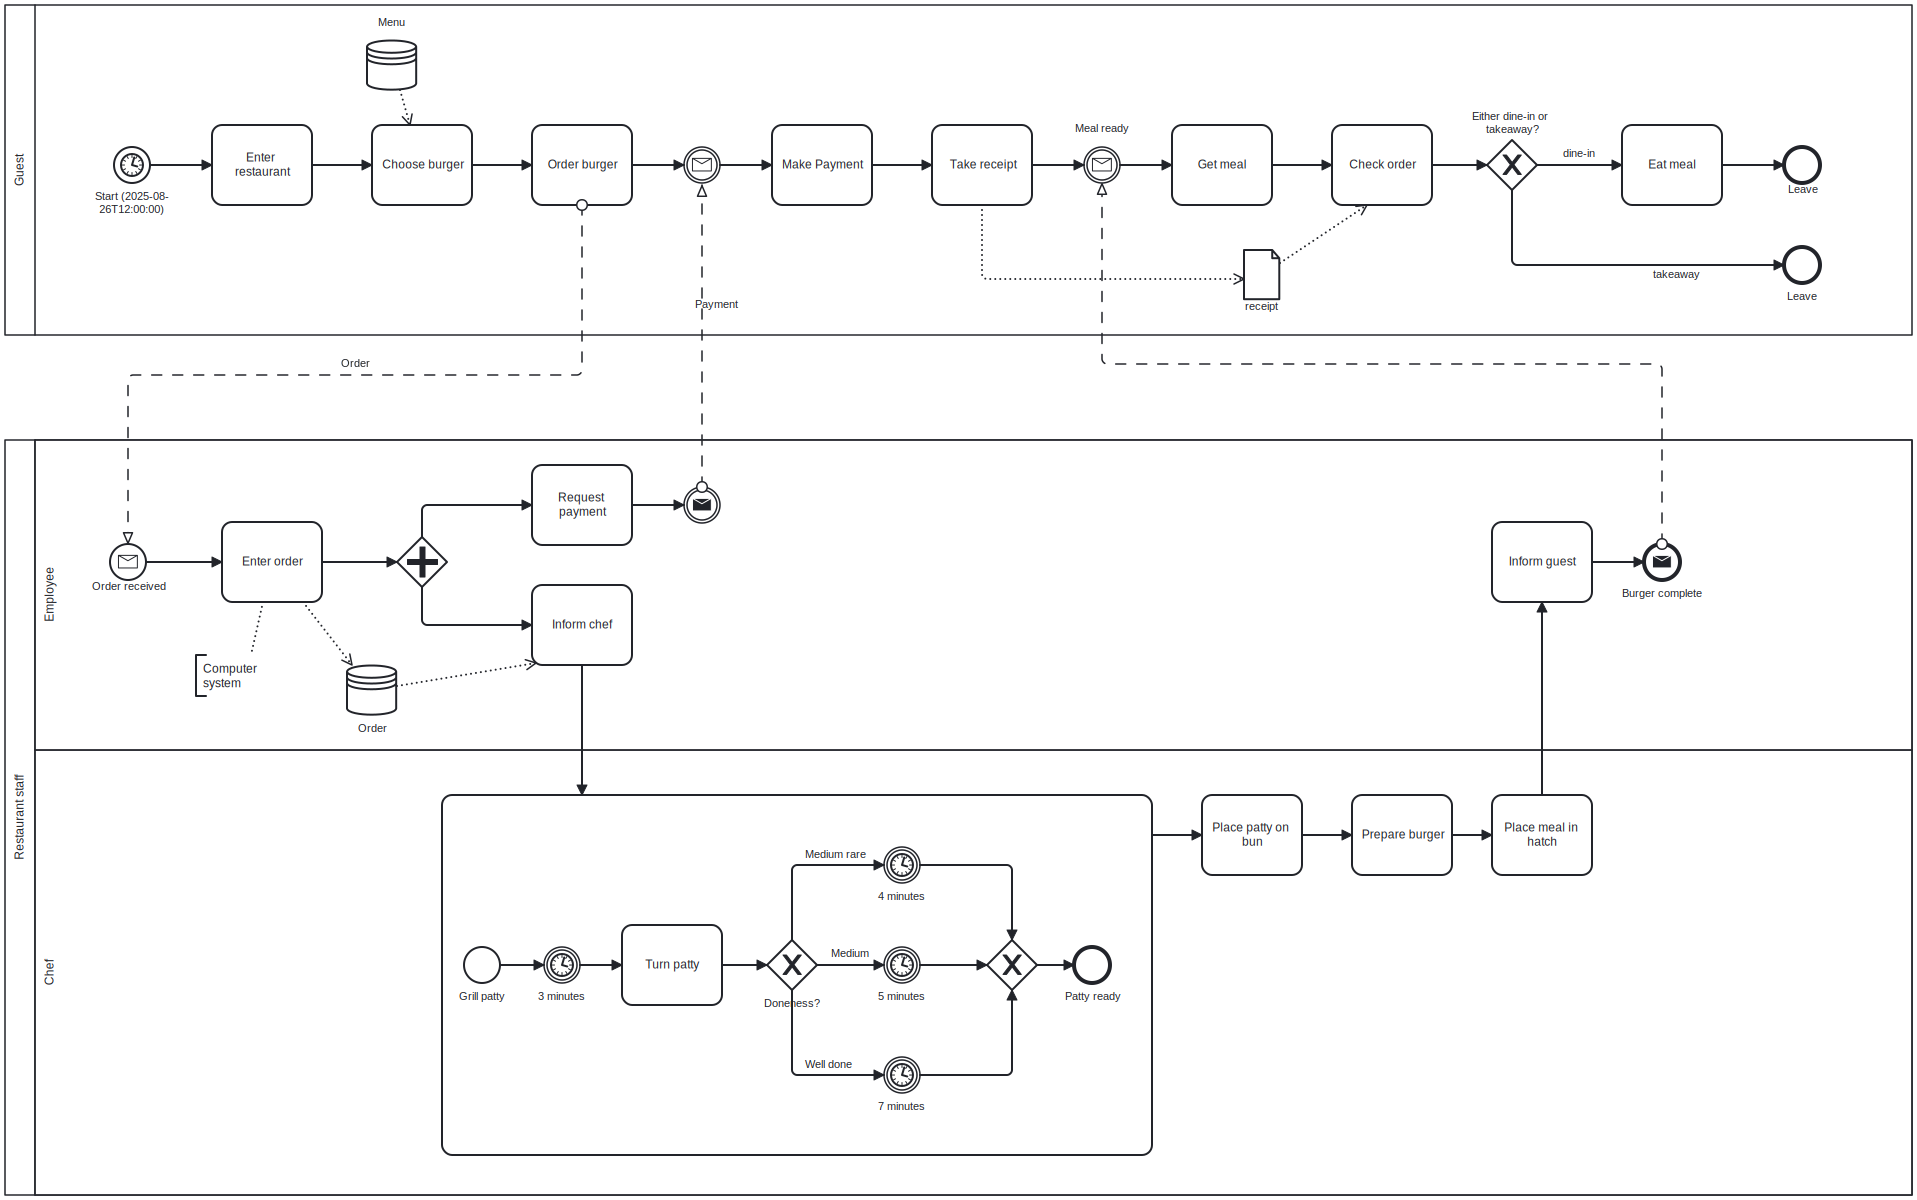
\includegraphics[width=\textwidth]{images/diagrams/diagram_0}
    \label{fig:bpmn-elements}
    \caption{BPMN 2.0\cite{omg2014bpmn2} Diagramm mit allen relevanten Elementen}
  \end{figure}


Für die Chatbot-Implementierung ist das Verständnis dieses Systems entscheidend, 
da alle Elemente diesen Konventionen entsprechen müssen, damit sie 
in bpmn.js korrekt dargestellt werden. 


\section{Large Language Models}

Large Language Models (LLMs) sind Systeme, die auf der Verarbeitung und Generierung 
natürlicher Sprache spezialisiert sind. 
Das Konzept wurde 2017 von Vaswani et al.\cite{vaswani2023attentionneed} eigeführt.
Sie basieren auf \texttt{Deep-neural Networks}, insbesondere auf Transformer-Architekturen, die große 
Mengen an Textdaten analysieren, um Muster, Strukturen und Zusammenhänge in der Sprache zu erkennen. 
Durch dieses Training können LLMs sowohl Texte verstehen als auch neue Texte generieren.

Ein LLM wird typischerweise durch überwachtes Lernen trainiert, wobei 
das Ziel darin besteht, das nächste Wort oder den nächsten Satz in einem gegebenen Kontext korrekt 
vorherzusagen. 
Moderne LLMs, wie GPT-Modelle, verfügen über Milliarden von Parametern, die ein 
Sprachverständnis und die Fähigkeit zur Textgenerierung besitzen.

Die Anwendungsbereiche von LLMs sind vielfältig. Sie reichen von Textgenerierung, Übersetzungen und 
Zusammenfassungen über Frage-Antwort-Systeme bis hin zu Chatbots und automatisierten 
Prozessunterstützungen. 

LLMs können genutzt werden, um Geschäftsprozesse in BPMN-Diagramme zu überführen. 
Dazu analysiert das Modell natürliche Sprache, wie z.B. Prozessbeschreibungen, 
Anweisungen oder Anforderungen, und 
wandelt diese in strukturierte BPMN-Elemente wie Tasks, Events, Gateways, Pools und Lanes um. 
LLMs können dabei sowohl die logische Abfolge der Prozessschritte erkennen als auch Verzweigungen 
und Kommunikationsflüsse zwischen Beteiligten identifizieren.

In der Praxis erfolgt dies oft in Form einer Text-zu-BPMN-Übersetzung, bei der das LLM die 
Prozessinformationen in eine JSON- oder XML-Repräsentation überführt, die anschließend von Tools 
wie bpmn.js visualisiert werden kann. 
Auf diese Weise können LLMs die Erstellung von Prozessmodellen erheblich beschleunigen, 
Standardisierung fördern und auch komplexe Abläufe automatisch konsistent darstellen.

\section{Chain of Thought}

Chain of Thought beschreibt eine Methode, bei der ein Large Language Model (LLM) seine 
Gedankenschritte offenlegt und erklärt, wie es zu einer bestimmten Antwort kommt. 
Statt nur ein Ergebnis zu liefern, zeigt das Modell also den Weg dorthin, ähnlich wie ein Mensch, 
der seine Überlegungen laut ausspricht. 
Diese Vorgehensweise ist besonders hilfreich bei Aufgaben, die mehrere Denkschritte erfordern, 
etwa beim Lösen von Problemen, beim Strukturieren von Informationen oder beim Verstehen komplexer 
Anweisungen.
Diese Vorgehensweise wurde von Wei et al.\ grundlegend untersucht
~\cite{wei2023chainofthought}.

Im Kontext der Unterhaltung zwischen Mensch und KI führt Chain of Thought dazu, dass das Modell 
transparenter und nachvollziehbarer reagiert. 
Die KI kann Gedankengänge ausformulieren, Entscheidungen begründen und schwierige Themen Schritt 
für Schritt erklären. 
Dadurch entsteht ein natürlicherer Dialog, da der Benutzer nicht nur das Ergebnis sieht, sondern 
auch versteht, wie die KI dorthin gelangt ist. 
Gleichzeitig hilft diese Technik dem Modell selbst, bessere Antworten zu geben, weil es 
Zwischenschritte bewusster berücksichtigt und Fehler eher vermeiden kann.

Für die Erstellung von BPMN-Diagrammen ist diese Vorgehensweise besonders wertvoll. 
BPMN erfordert eine klare Struktur von Ereignissen, Aufgaben, Gateways und Abläufen. 
CoT ermöglicht es ChatGPT, Prozessbeschreibungen in einzelne Handlungsschritte zu zerlegen, diese 
sinnvoll anzuordnen und anschließend die passenden BPMN-Elemente daraus abzuleiten. 
So lässt sich Schritt für Schritt erarbeiten, welche Tasks benötigt werden, wo Entscheidungen 
auftreten und wie die Kommunikation zwischen Rollen oder Abteilungen abgebildet werden muss. 
Chain of Thought macht die Diagrammerstellung dadurch deutlich präziser, transparenter und 
konsistenter.

\section{Streaming}

Streaming bezeichnet die kontinuierliche Übertragung von Daten zwischen einem Sender und einem 
Empfänger, wobei die Daten in aufeinanderfolgenden Teilen statt als komplette Datei oder Nachricht 
übertragen werden. 
Dieses Verfahren ermöglicht es, dass Informationen bereits während der Generierung oder Übertragung 
verarbeitet und angezeigt werden können, wodurch die Latenz für den Nutzer deutlich reduziert wird. 
Streaming findet Anwendung in vielfältigen Bereichen, etwa bei Audio- und Videoinhalten, 
Live-Datenübertragungen oder auch der Ausgabe von Ergebnissen von KI\@. 
Wie dieses Streaming effizient umgesetzt werden kann, wurde von Xiao et al.\ bei der 
International Conference on Representation Learning 2024 (ICLR 2025)\cite{iclr2024streaming}
gezeigt.
Technisch basiert Streaming häufig auf asynchronen Datenströmen, bei denen die empfangenen Daten in 
Echtzeit analysiert und weiterverarbeitet werden. 
Zu den verbreiteten Übertragungsprotokollen zählen HTTP-basierte Verfahren wie 
Server-Sent Events (SSE)\cite{fette2011sse}
oder WebSockets, die eine kontinuierliche, bidirektionale Kommunikation ermöglichen. 
Insgesamt steigert Streaming die Geschwindigkeit der Datenverarbeitung und verbessert die Nutzererfahrung 
durch eine Anzteige des aktuellen Zustands in Echtzeit.

Im Kontext von KI-Systemen ermöglicht Streaming die Übersendung von Modellantworten an 
den Nutzer, noch während die Generierung der Daten läuft. 
Dies ist besonders relevant bei Modellen, die unter anderem auch Text erzeugen. 
Technisch erfolgt dies meist über asynchrone Streams, die Datenpakete kontinuierlich übertragen.
Die Textfragmente werden hier in der Regel auch \texttt{Delta} genannt.
Auf diese Weise lässt sich die Benutzererfahrung deutlich verbessern, da Rückmeldungen sofort sichtbar 
sind und Wartezeiten minimiert werden. 

\section{Base64}

Base64 ist ein Kodierungsverfahren, das Binärdaten in eine reine Textdarstellung überführt, 
um sie über textbasierte Protokolle wie HTTP mit unter anderem JSON zuverlässig übertragen 
zu können. 
Da viele APIs und Webschnittstellen ausschließlich Text unterstützen oder die Übermittlung 
binärer Inhalte erschweren, bietet Base64 eine Möglichkeit, Dateien plattformunabhängig und 
ohne zusätzliche Infrastruktur weiterzugeben. 
Die Kodierung funktioniert, indem jeweils 24 Bit (drei Byte) in vier 6-Bit-Gruppen umgewandelt 
und anschließend als ASCII-Zeichen dargestellt werden. 
Dadurch vergrößert sich die Datenmenge zwar um etwa ein Drittel, sie wird jedoch vollständig 
textkompatibel.\cite{rfc4648}

Im Kontext von Webanwendungen werden Base64-kodierte Inhalte häufig in Form sogenannter 
\texttt{Data URL}s\cite{rfc2397} übertragen. 
Eine Data URL bettet die kodierten Daten direkt in einen einzigen Zeichenstring ein, der aus 
vier Komponenten besteht: 
\begin{enumerate}
    \item einem Präfix zur Typangabe (data:)
    \item dem MIME-Typ der Datei (z. B. image/png;)
    \item der Kodierungsart (base64)
    \item dem eigentlichen Datenbereich
\end{enumerate}
Eine Data URL mit Base64 Encoding entspricht somit typischerweise der Form
\verb|data:<mime-type>;base64,<kodierte-daten>|. 
Browser und APIs können diese Darstellung unmittelbar wieder in eine gültige Datei 
zurückkonvertieren, ohne dass separate Dateipfade, temporäre Speicherorte oder Upload-Endpunkte 
notwendig sind.

Für KI-Systeme stellt dieses Verfahren einen effizienten Weg dar, Dateien wie 
Bilder oder Dokumente direkt in die Prompt-Struktur zu integrieren. 
Die Base64 Data URL kann als gewöhnlicher String an das Backend übermittelt und ohne weiteren 
Zwischenschritt an die API des KI-Anbieters weitergereicht werden. 
Dies reduziert die Komplexität der Implementierung und ermöglicht eine 
Unterstützung verschiedener Dateitypen. 
Durch diese Eigenschaften eignet sich Base64 in Kombination mit Data URLs optimal für eine 
unkomplizierte Übertragung von Dateien innerhalb von KI basierten Anwendungen.

\section{Reflective Prompting}

Reflective Prompting ist eine Strategie, bei der ein KI-Modell dazu 
aufgefordert wird, seine eigenen Ergebnisse zu überprüfen.
Im Gegensatz zum klassischen Prompting, das direkt eine fertige Ausgabe erzeugt, arbeitet 
Reflective Prompting in zwei voneinander getrennten Phasen: 
Zunächst erstellt das Modell einen ersten Entwurf, eine interne Einschätzung oder einen 
vorläufigen Vorschlag. 
Anschließend reflektiert das Modell diesen Entwurf, prüft auf mögliche Fehler, Unklarheiten 
und logische Inkonsistenzen und verbessert daraufhin die Antwort.\cite{zhao2024factandreflection}

Durch die Einbeziehung einer Reflexionsphase steigt die Wahrscheinlichkeit, dass 
das Modell eigene Ungenauigkeiten erkennt, fehlende Teile ergänzt und konsistentere 
und qualitativ bessere Ergebnisse liefert. 
Reflective Prompting hat sich insbesondere bei Aufgaben bewährt, die mehrstufiges Denken, 
komplexe Entscheidungsfindung oder strukturiertes Argumentieren erfordern.

Gleichzeitig bringt diese Technik auch Herausforderungen mit sich. 
Da das Modell zusätzliche Denk- und Analyseprozesse durchläuft, erhöht sich sowohl die 
Rechenzeit als auch der Tokenverbrauch. 
Dennoch überwiegt in vielen Anwendungsszenarien der Qualitätsgewinn. 
In der Forschung zu Large Language Models wird Reflective Prompting daher zunehmend als 
zentrale Methode betrachtet, um Fehlerraten zu senken und die Robustheit der 
Antworten zu verbessern.

\section{BPMN-Gen}

BPMN-Gen ist ein Projekt der Universität Ulm, Institut für Datenbanken und Informationssystem.
Das Projekt wurde von Weidl~\cite{weidl2024bpmngen} gestartet, von Shi~\cite{shi2025bpmngen} fortgeführt und 
von weiteren Personen und Gruppen weiterentwickelt.
Es geht in dem Projekt darum einen LLM basierten Chatbot zu entwickeln, welcher möglichst interaktiv Prozessbeschreibungen 
in BPMN 2.0 Diagramme umwandeln kann.
Dieser Chatbot ist als Webanwendung
\footnote{Die Anwendung ist verfügbar unter \url{https://bpmngen.de}} und als Rest-API implementiert.

\subsection{Frontend}

Das Frontend ermöglicht es den Nutzerinnen und Nutzern, mit dem BPMN-Gen System zu interagieren.
Die Grundidee besteht darin, BPMN Diagramme über Chat Interaktionen mit verschiedenen KI Modellen zu generieren.
Nutzer können sich über eine Login- und Registrierungsseite anmelden.
Nach dem Login erhalten sie Zugriff auf ein Dashboard, in dem sie
neue Chats erstellen, bestehende Chats anzeigen, verwalten und fortsetzen können.
Dabei haben sie die Möglichkeit, zwischen verschiedenen KI Modellen, Ausgabeformaten und Modi für die BPMN Diagrammgenerierung zu wählen.
Zusätzlich können Dateien als Eingabe für die KI Modelle bereitgestellt werden, beispielsweise bereits vorhandene BPMN Diagramme.
Die Chat Interaktion kann sowohl über Texteingabe als auch über Spracheingabe erfolgen.
Das Frontend ist mit Angular umgesetzt und nutzt die Bibliothek bpmn-js zur Darstellung und Bearbeitung von BPMN Diagrammen.

In dieser Arbeit wird nicht weiter auf das Frontend eingegangen, sondern fokusiert ausschließlich auf dem Backend.

\subsection{Backend}

Das Backend stellt den Zugriff auf mehrere KI-APIs, sowie eine Nutzer- und Threadverwaltung bereit.
Die Implemtierung ist darauf ausgelegt, BPMN-Diagramme aus Benutzereingaben zu generieren. 
Diese Eingaben können in Form von Text, Bildern, Dokumenten oder natürlicher Sprache erfolgen.
Der Server kann Create- und Update-Anfragen für Diagramme entgegennehmen und leitet diese an die KI-API weiter.
Die Antwort des Servers hängt dabei vom gewählten KI-Modell und dem angeforderten Ausgabeformat ab.
Alle generierten Diagramme werden in einer durch Prisma erzeugten Postgres Datenbank gespeichert.
Das Backend basiert auf Express.js, welches als Webserver Framework für die Verarbeitung von 
HTTP-Anfragen, Routing und Middleware eingesetzt wird.

\section{Thread}

Ein Thread ist ein fortlaufender Gesprächsverlauf zwischen einem Nutzer und einem KI-Modell. 
In einem Thread werden alle Nachrichten, also Fragen, Antworten und Kontext, gespeichert, 
sodass das Modell den Zusammenhang früherer Beiträge berücksichtigen kann. 
Dadurch kann die KI besser reagieren, sich auf bereits Gesagtes beziehen und ein Gespräch 
weiterführen, anstatt jede Anfrage isoliert zu behandeln.